\documentclass[a4paper, 11pt]{article}
\usepackage{comment}
\usepackage{amsmath}
\usepackage{mathtools}
\usepackage{fullpage}
\usepackage{graphicx}
\graphicspath{ {images/} }


\begin{document}
\title{ CSE 519 -Homework 3 Report}
\author{Amol Damare \\ adamare@cs.stonybrook.edu \\Sbu Id : 107914028
\and
Punit Mehta\\ Punit.Mehta@stonybrook.edu \\Sbu Id: 111461860}

\maketitle
\section{Goal}
The goal of this homework assignment is to improve upon the models we built in homework 2 for Zillow's kaggle competition. In this assignment we will learn about how to systematically approach the data science problem and employ various statistical tools to improve upon a baseline model. In this assignment we have improved upon our previous models. This report will explain our approach and reasoning behind all the tasks that we did. In first section we will give a brief overview of what tasks we did in homework 2. In next section we will present the our ideas for improvement and reasoning behind these ideas. Lastly we will present our results and evaluation of our models
\section{Previous work}
In last homework we designed a simple linear model and used data given by Zillow to predict the "logerror". In the assignment we hand picked the features removed any missing values and used this basic cleansed data to fit the model. We used residual graphs to evaluate this model. Table \ref{table:1} presents the results of this model. This model also scored  0.0674213 on Zillow's competition. As we can see from the score we obtained there is still room to improve this model. In this assignment we will attempt improve this model. 
\begin{table}[h!]
\centering
\begin{tabular}{||c c c ||} 
 \hline
 Data Set & Training &  Testing \\ [0.5ex] 
 \hline\hline
 Mean Square Error & 0.0285  & 0.0275 \\ [1ex] 
 \hline
\end{tabular}
\caption{Mean square errors for linear regression model in homework 2}
\label{table:1}
\end{table}
\\
Before we discuss the improvement methods we used, let's discuss the issues with our previous model.
\subsection{Issues with previous model}
In the previous model we did not do any extensive data cleaning. We neither normalized or scaled the data. Only cleaning task we did was to remove missing entries. Other main issue with previous assignment we did was we used features that we thought would work well. There was no statistical reasoning behind this selection. If we could rectify these issues then we think we will be able to improve our model.The next section will present the ideas we used to improve the model and our reasoning behind these ideas.
\section{Improvement Tasks}
One of the first things we thought of improvement was selection features based some statistical evidence.
\subsection{Feature Selection}
Zillow data has 57 features for a given property. We want to select the best features among these to consider for our models. One of the ways we can do this is by using feature selection algorithms. There are various selection algorithms that can be used. We can eliminate the features which has very low variance, as low variance means that this feature doesn't convey a lot of information. And feature has similar values for most of the data points. Another way we can eliminate the features is using univariate feature selection algorithms which uses univariate statistical tests such as $X^2$.\\
In this experiment, however, we are going to use sklearn's SelectFromModel feature selection algorithm. It uses an estimator and selects the features having weights or coefficients only above a specified threshold. Thresholds can be specified numerically or they can be determined heuristically by sklearn library. We are going to use Lasso regression for selecting the features. But before we could do that, we have to prepare our data to be used for regression
\subsection{Data cleaning and preparation}
To get good results from feature selection algorithms it is recommended that all variables should be normalized and scaled. Since we are using lasso regression for feature selection we can skip scaling of the data. Following are the steps we used to get clean and prepare the data for feature selection.
\begin{enumerate}
\item Encode all the categorical variables. This step is necessary to perform in regression.
\item Impute missing values in the data. In this step we just replaced missing values with mean. (We did try removing them but results were not that good).
\item Normalize the data set.

\end{enumerate}
After these steps we applied feature selection algorithm to get the best possible features we can use for our model. We got 17 features out of 57 as a result of feature selection algorithm. We will now present our experiment and evaluation of our models.
\section{Experiment and Evaluation}
We used 2 models in this experiment. We wanted to know if we have improved our baseline linear regression model by using feature selection. And we also wanted to test a complex model, so we choose random forest regression. Random forest regression is an ensemble learning method in which multiple decision trees are created at training time and a value is predicted using these decision trees. We think this model will work best with the features we have chosen since the features have very less covariance between them and all of the features are normalized so we all the trees in random forest will have similar weights. We trained these 2 models using the Zillow data we obtained after applying the cleaning steps we performed. In next section we will present the evaluations of these models.
\subsection{Evaluation}
As expected linear model improved after performing the data cleaning and feature selection.  Table \ref{table:2} shows the training and testing errors for the linear model. This model has $r^2$ score of 0.04 which indicates that model is good. 
\begin{table}[h!]
\centering
\begin{tabular}{||c c c ||} 
 \hline
 Data Set & Training &  Testing \\ [0.5ex] 
 \hline\hline
 Mean Square Error & 0.0264  & 0.0238 \\ [1ex] 
 \hline
\end{tabular}
\caption{Mean square errors for linear regression model in homework 3}
\label{table:1}
\end{table}
Figure \ref{fig:res1} shows the residual graph of our linear regression model. We also performed permutations test for the linear model. Figure \ref{fig:res2} shows the result of permutation test for linear model. As our $pvalue<0.005$, we can reject the null hypothesis which is that our model is as good as random prediction. So we can say that our linear model is a sound model and does a fairly well job of predicting the logerror. We have submitted this model's result to zillow competition on kaggle.
Linear model worked well and improved our previous model on kaggle. We got score of 0.0655138 which was improvement over our previous homework's submission which scored 0.0659056.
\begin{figure}[h]
    \centering
    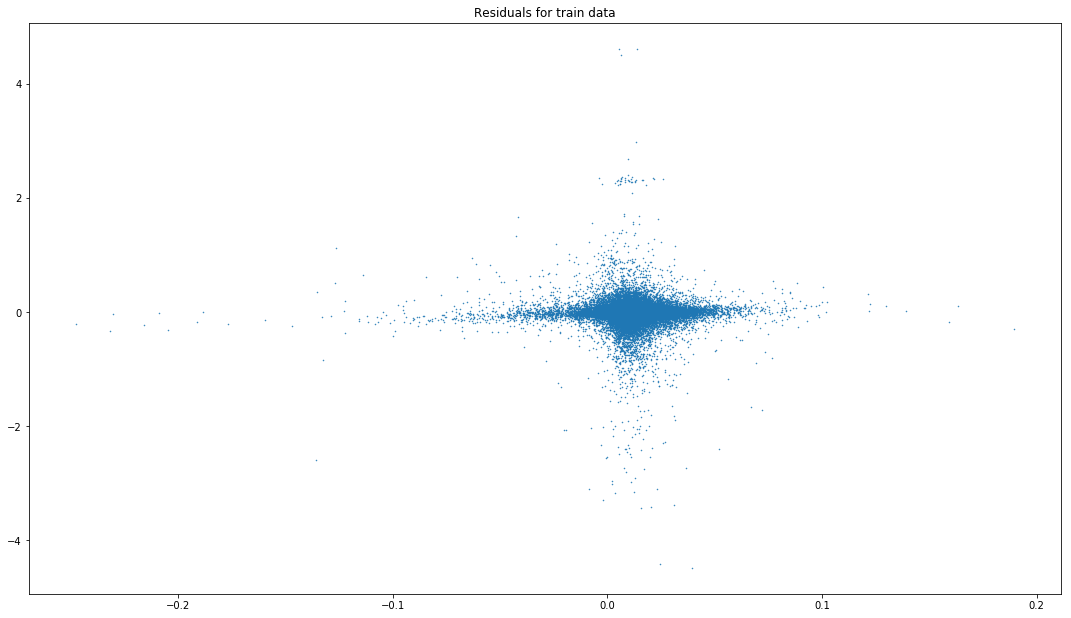
\includegraphics[width=0.75\textwidth]{residual}
    \caption{Residual plot for linear regression model }
    \label{fig:res1}
\end{figure}
\begin{figure}[h]
    \centering
    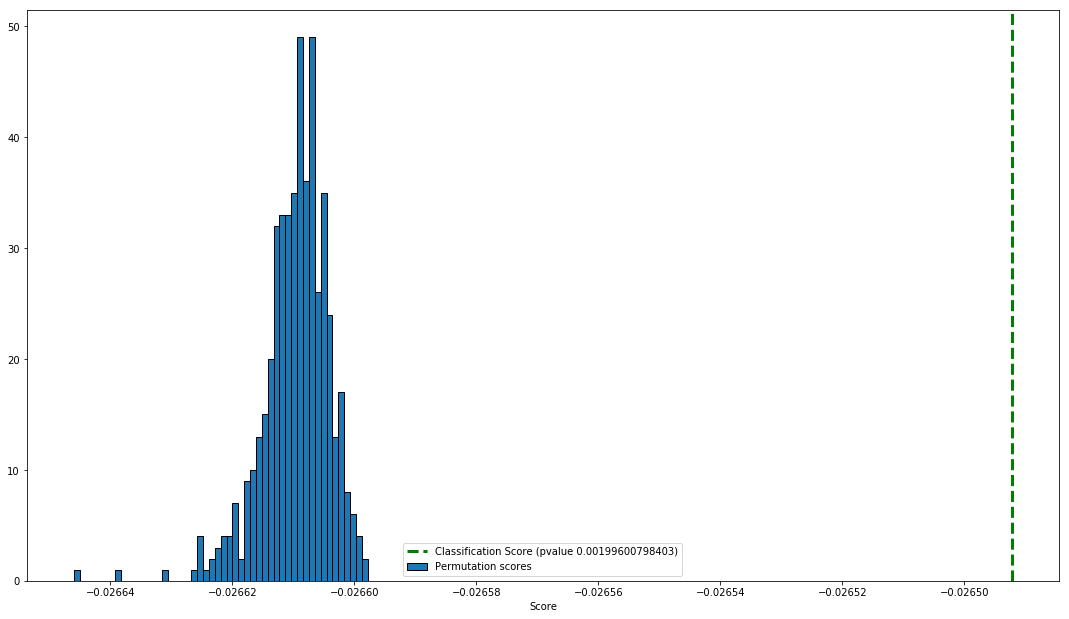
\includegraphics[width=0.55\textwidth]{ptest_linear}
    \caption{Permutation test for linear regression model }
    \label{fig:res2}
\end{figure}
We will now present the evaluation of our random forest model. Table \ref{table:3} gives the mean error values of this model. This model gives us similar results to that of linear regression. Figure \ref{fig:res3} shows result of permutation test for random forest model. As you can see from permutation tests this model is worse. P-value is 0.67 so half the time it works same as giving a noise output for prediction. It seems from the p-test that the above model might not be best one considering the features we took to solve this problem.
\begin{table}[h!]
\centering
\begin{tabular}{||c c c ||} 
 \hline
 Data Set & Training &  Testing \\ [0.5ex] 
 \hline\hline
 Mean Square Error & 0.0265  & 0.0239\\ [1ex] 
 \hline
\end{tabular}
\caption{Mean square errors for random forest model in homework 3}
\label{table:3}
\end{table}
\begin{figure}[h]
    \centering
    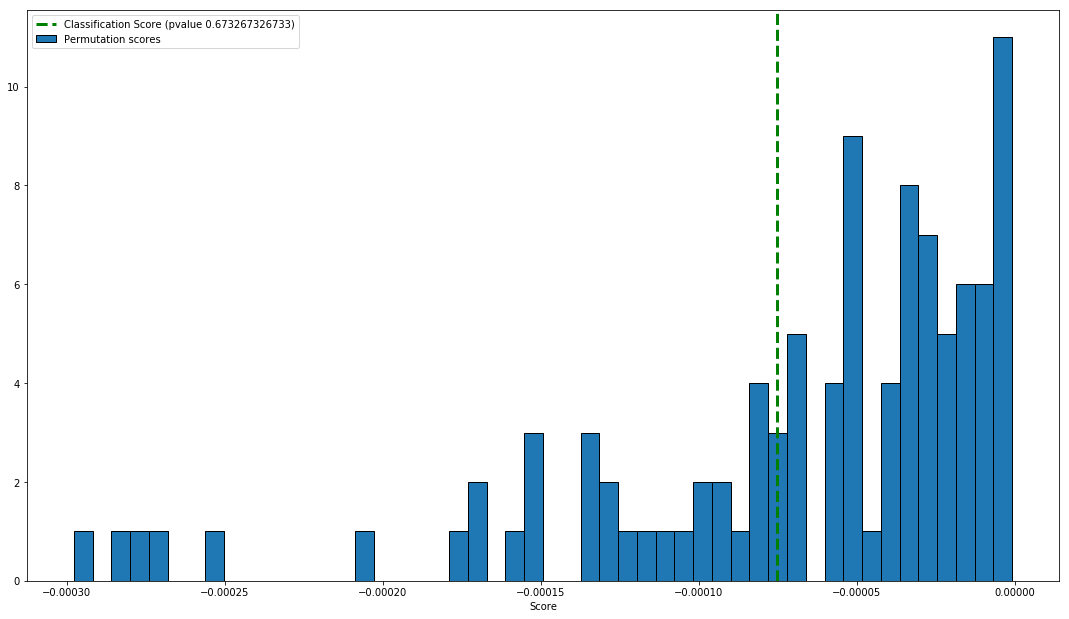
\includegraphics[width=0.75\textwidth]{ptest_rf}
    \caption{Permutation test for random forest model }
    \label{fig:res3}
\end{figure}
\section{Conclusion}
In this assignment we learned various techniques we can apply to improve our models. And it takes careful evaluation of choices we make in data cleaning that leads to improvement of a model. We also learned about use of permutation test in evaluation of the models
\begin{thebibliography}{9}
\bibitem{1} Steven Skiena ,\emph{The Data Science Design Manual} ,2017,Springer International Publishing.
\bibitem{2}  Kaggle Zillow Challenge, \emph{https://www.kaggle.com/c/zillow-prize-1}
\bibitem{3}  Linear Regression Wikipedia article, \emph{https://en.wikipedia.org/wiki/Linear\_regression}
\bibitem{4} Sci-kit learn package for Python, \emph{http://scikit-learn.org/stable/}
\bibitem{5} Pandas package for python,\emph{http://pandas.pydata.org/}
\bibitem{6} Sci-kit learn SVM tutorial, \emph{http://scikit-learn.org/stable/modules/svm.html}
\end{thebibliography}
\listoffigures
\listoftables
\end{document}
